\documentclass{beamer}

% Choose how your presentation looks.
\mode<presentation>
{
\usetheme{Darmstadt}      % or try Darmstadt, Madrid, Warsaw, ...
\usecolortheme{wolverine} % or try albatross, beaver, crane, ...
\usefonttheme{structurebold}  % or try serif, structurebold, ...
\setbeamertemplate{navigation symbols}{}
\setbeamertemplate{caption}[numbered]

%Customerize Prasentation
\definecolor{Grau}{HTML}{CCCCCC}
\definecolor{GrauDark}{HTML}{777777} % auf weißem hintergrund
\definecolor{Orange}{HTML}{EA5B10}
\setbeamercolor{palette primary}{bg=Grau}
\setbeamercolor{palette primary}{fg=Orange}
\setbeamercolor{normal text}{fg=GrauDark}
\setbeamercolor{structure}{fg=Orange} % farbe der items
\setbeamertemplate{itemize item}[circle]
\setbeamercolor{mini frame}{fg=Orange}
\setbeamercolor{section in head/foot}{bg=Grau}
\setbeamercolor{section in head/foot}{fg=Orange}
\setbeamercolor{subsection in head/foot}{bg=white}
\setbeamercolor{subsection in head/foot}{fg=GrauDark}
\setbeamercolor{headline}{bg=Grau}
\setbeamercolor{block body}{bg=white}
\setbeamercolor{frametitle}{bg=white}
}

\usepackage[utf8]{inputenc}
\usepackage[T1]{fontenc}
\usepackage{ae}
\usepackage{ngerman}
\usepackage{calc}
\usepackage{graphicx}
\usepackage{makecell}
\usepackage{pgfplots}
\usepackage[autostyle=true,german=quotes]{csquotes}
\pgfplotsset{compat=1.4}

\newenvironment<>{varblock}[2][.9\textwidth]{%
  \setlength{\textwidth}{#1}
  \begin{actionenv}#3%
    \def\insertblocktitle{#2}%
    \par%
    \usebeamertemplate{block begin}}
  {\par%
    \usebeamertemplate{block end}%
  \end{actionenv}}


\title{FreeJDAQ}
\subtitle{Visuelle Programmiersprache zur Datenerfassung auf
einem Raspberry Pi}
\author{David Gawron, Stefan Geretschlaeger, Leon Huck,
Jan Kublbeck, Linus Ruhnke }
\date{23.09.2019}

\begin{document}

\begin{frame}
\titlepage
\end{frame}

\section{Einleitung}

\begin{frame}{Einleitung}
\frametitle{Problemstellung}
	\begin{figure}[htbp]
    	\begin{center}
       	 
\includegraphics[width = 5cm]{Grafiken/FreeJDAQ.png}
    	\end{center}
	\end{figure}
\end{frame}

\begin{frame}{Einleitung}
\frametitle{Abgrenzungen}
\end{frame}

\section{Softwaretechnik}

\begin{frame}{Softwaretechnik}
\frametitle{Grundaufbau}
\end{frame}

\begin{frame}{Softwaretechnik}
\frametitle{Paketdiagramm}
\begin{figure}[htbp]
    	\begin{center}
       	 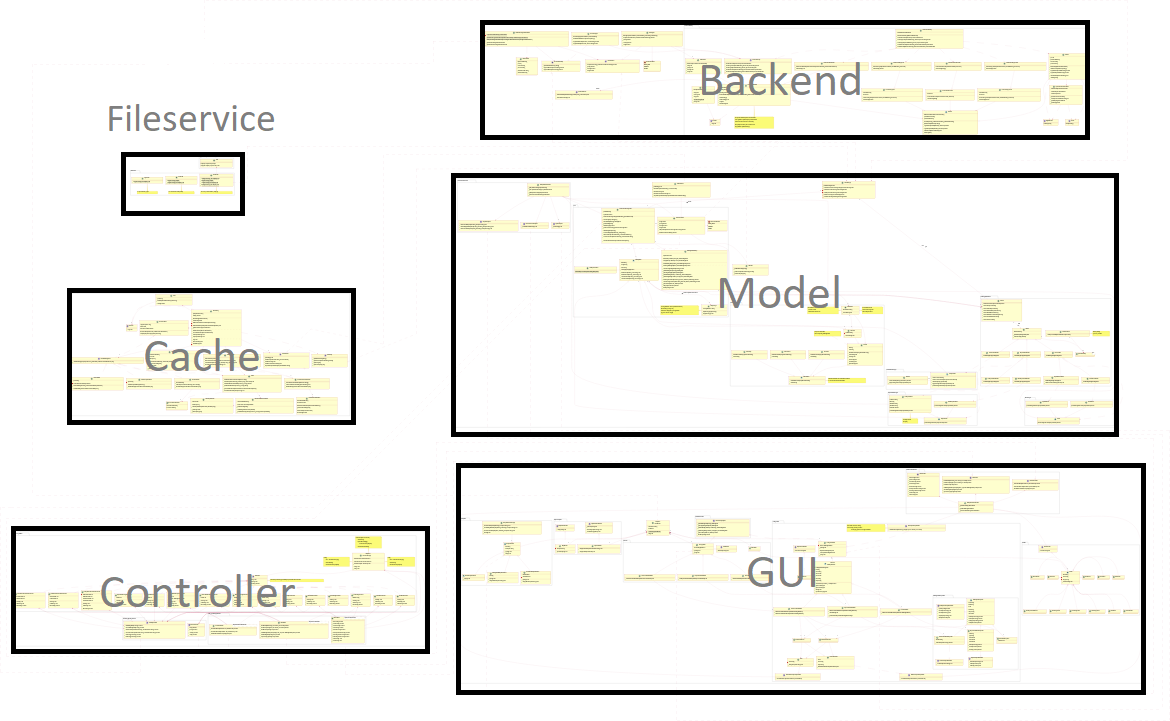
\includegraphics[width = 10cm]{Grafiken/Klassendiagramm.png}
    	\end{center}
	\end{figure}
\end{frame}

\section{Statistiken}

     \begin{frame}{Unit-Tests}
    \centering
    \begin{tikzpicture}
    \begin{axis}[
    ybar,
    enlarge x limits=0.2,
    width=0.95\textwidth,
    height=0.8\textheight,
    ylabel={Anzahl},
    xtick=data,
    nodes near coords,
    ymin=0,
    legend pos=north west,
    xticklabel style={rotate=45},
    symbolic x coords={GUI,Model,Controller,Backend,Cache,FileService},xticklabels={GUI,Model,Controller,Backend,Cache,FileService},
    ]
    
    \addplot coordinates
    {(GUI,17) (Model,64) (Controller,100) (Backend,74) (Cache,36) (FileService,16)};
    \end{axis}
    \end{tikzpicture}
    Insgesamt 215 Testcases
\end{frame}

\begin{frame}{Statistiken}
\frametitle{Testabdeckung}
  \centering
    \begin{tikzpicture}
    \begin{axis}[
    ybar,
    enlarge x limits=0.2,
    width=0.95\textwidth,
    height=0.8\textheight,
    ylabel={Prozentl},
    xtick=data,
    nodes near coords,
    ymin=0,
    legend pos=north west,
    xticklabel style={rotate=45},
    symbolic x coords={Controller,FileService,GUI,Cache,Model,Backend},xticklabels={Controller,FileService,GUI,Cache,Model,Backend},
    ]
    
    \addplot coordinates
    {(Controller,53) (FileService,79) (GUI,84) (Cache,84) (Model,85) (Backend,96)};
    \end{axis}
    \end{tikzpicture}
    Insgesamt 80 Prozent
\end{frame}

\begin{frame}{Statistiken}
\frametitle{GitHub- FreeJDaq}
\begin{figure}[htbp]
    	\begin{center}
       	 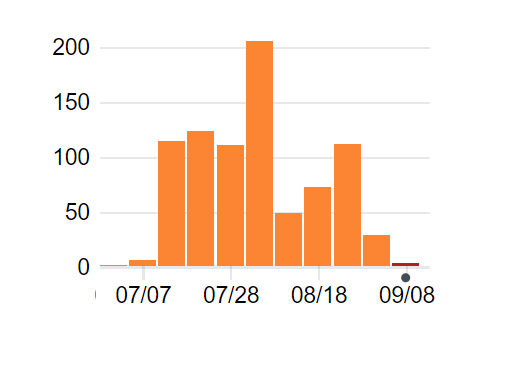
\includegraphics[width = 9cm]{Grafiken/Commits.png}
    	\end{center}
\end{figure}
\end{frame}

\begin{frame}{Statistiken}
\frametitle{GitHub- DAQDocuments}
\begin{figure}[htbp]
    	\begin{center}
       	 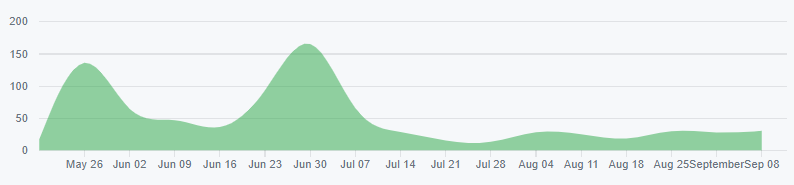
\includegraphics[width = 12cm]{Grafiken/CommitsDAQDocuments.png}
    	\end{center}
\end{figure}
\end{frame}

\begin{frame}{Statistiken}
\frametitle{GitHub- DAQDocuments}
\begin{figure}[htbp]
    	\begin{center}
       	 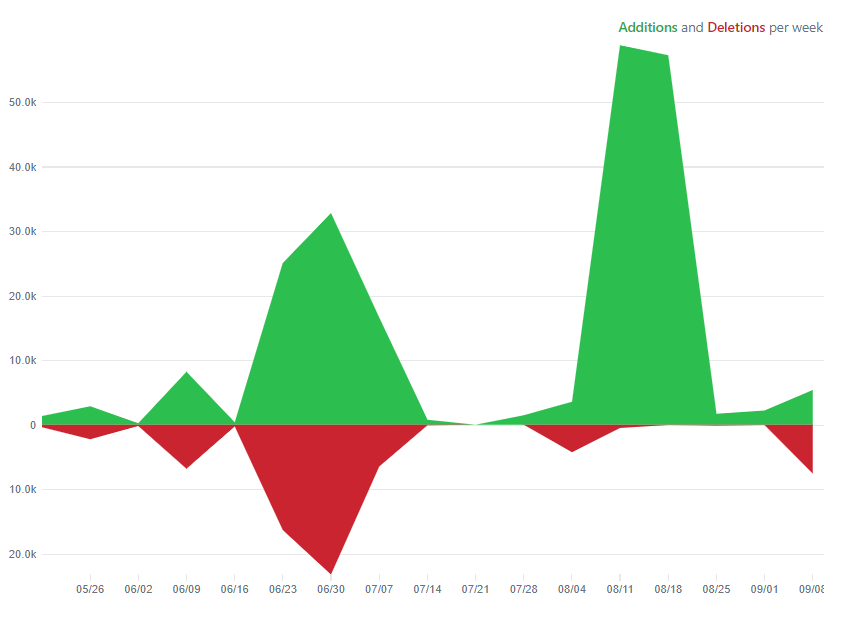
\includegraphics[width = 10cm]{Grafiken/DependencyGraphDAQDocuments.png}
    	\end{center}
\end{figure}
\end{frame}

\section{Tools}

\begin{frame}{Tools}
\frametitle{Allgemein}

 \begin{columns}
            \begin{column}{0.3\textwidth}
                \begin{block}{UML}
                    \center
                    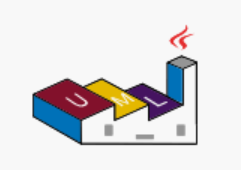
\includegraphics[width=(\textwidth / 2)]{Grafiken/PlantUmlIcon.png} %TODO find better logo
                \end{block}
            \end{column}
            \begin{column}{0.3\textwidth}
                \begin{block}{Unit-Testing}
                    \center
                    
\includegraphics[width=(\textwidth / 3)]{Grafiken/JUnitIcon.png}
                \end{block}
                \begin{block}{IDE}
                    \center
                    
\includegraphics[width=\textwidth / 4]{Grafiken/EclipseIcon.png}
                \end{block}
		   \begin{block}{Yaml-Editor}
		   \center
		   
\includegraphics[width=\textwidth]{Grafiken/SnakeYamlIcon.png}
                \end{block}
            \end{column}
                \begin{column}{0.3\textwidth}
                    \begin{block}{Continuous Integration}
                        
\includegraphics[width=(\textwidth)]{Grafiken/MavenIcon.png}
                    \end{block}
                    \begin{block}{Statische Codeanalyse}
                        \center
                        
\includegraphics[width=(\textwidth / 4)]{Grafiken/JacocoIcon.png}
                        
\includegraphics[width=(\textwidth / 2)]{Grafiken/EclEmmaIcon.png}
       	 	     
\includegraphics[width=(\textwidth / 2)]{Grafiken/SonarlintIcon.png}
                    \end{block}
                \end{column}
        \end{columns}
    \end{frame}

\section{Lernefahrung}

\begin{frame}
\frametitle{Probleme}
\end{frame}

\begin{frame}
\frametitle{Was haben wir gelernt}
\end{frame}

\end{document}